\subsection{Development Model}\label{sec:development}

To enable concurrent development across all the LSST DM sites, the development team uses a decentralized development model based on the Git version control system\footnote{\url{https://git-scm.com/}}.
[TODO: describe in terms of Agile values?]

\subsubsection{Version Control}\label{sec:git}\label{sec:subversion}

The choice of version control system has triggered many debates over the years but for DM with a distributed team working across multiple time zones it became clear in 2011 that DM should move its source code from Subversion to Git.
The advantages of Git over Subversion are well-documented, but one key advantage for a distributed team is the ability to work locally and make detailed commits without requiring that the remote server is always running.
It was decided that the best fit for our monolithic Subversion repository was to convert it to many individual Git repositories, as is common practice.

Initially we used gitolite for hosting git repositories on our own servers but in late 2014 we decided that we should move all development to GitHub\cite{Document-17187}.
DM was already a strong advocate of open development within LSST and this change made it considerably easier for the wider community to see what we were doing.
The move was completed by 2015 and whilst some developers were initially ambivalent about the change, after three years there is now a strong feeling that this was absolutely the correct decision and it has made it easier to leverage tools such as Travis, improved our code review abilities, and made it easier to link our pull requests to issues in other people's repositories.

\subsubsection{Code Organization}\label{sec:git_repositories}

The data management system is divided into several hundred individual Git repositories, hosted on GitHub\footnote{\url{http://github.com/lsst/} and \url{https://github.com/lsst-dm/}}.
Each repository corresponds to one code package, and all but a handful of repositories usually have at most one developer working on them at a time.
Isolating code in small repositories minimizes the need for developers to frequently download code updates, something the Git framework requires whenever developers make concurrent changes to the \texttt{master} branch of the same repository.
Representing each package by an independent repository also makes it easy to formalize and track inter-package dependencies using tools like EUPS (\autoref{sec:eups}).

\subsubsection{The LSST Workflow}\label{sec:dev_workflow}

\begin{figure}[t]
\begin{center}
  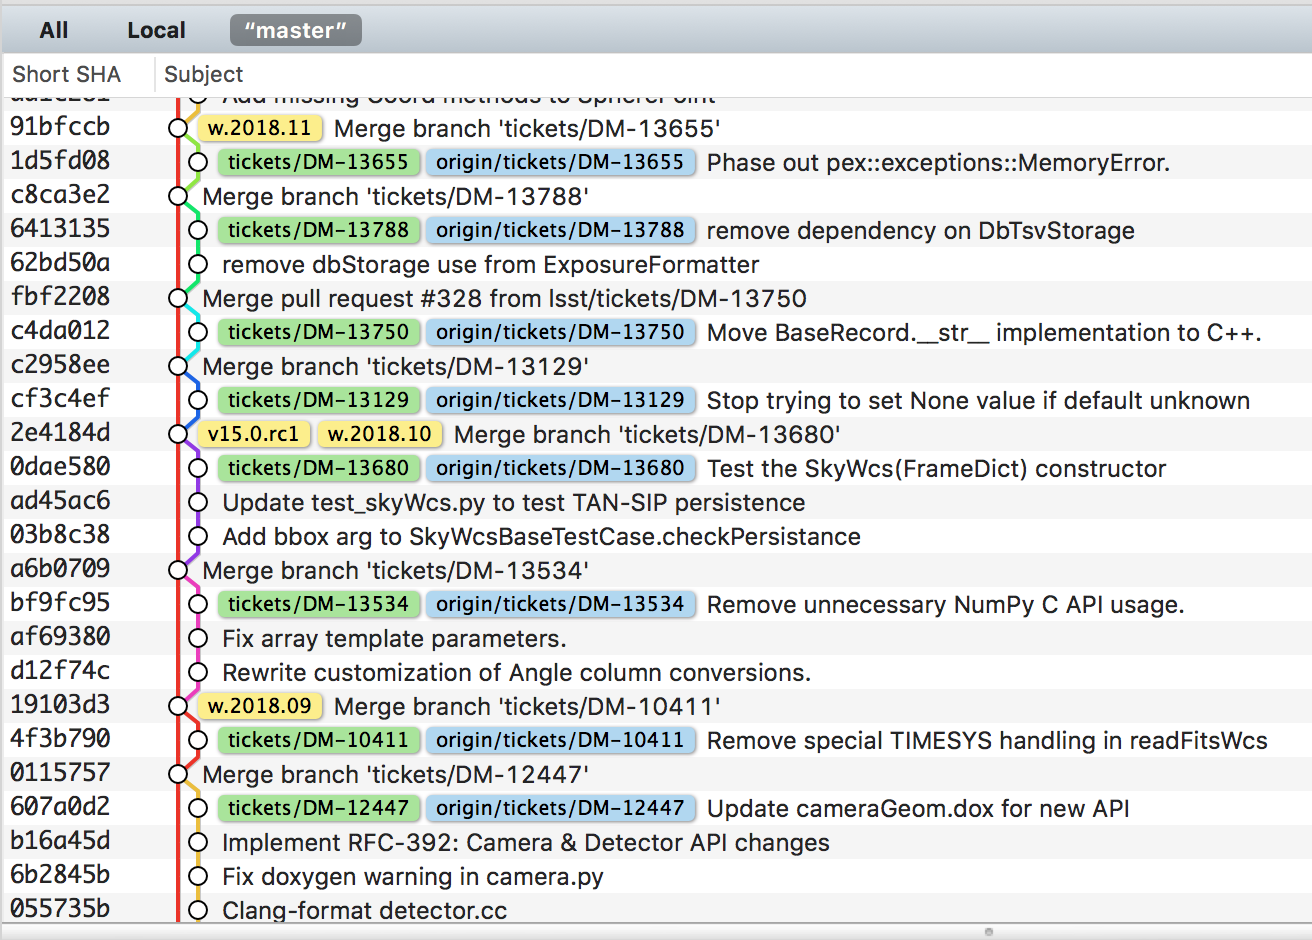
\includegraphics[width=0.7\textwidth]{git-history}
\end{center}
\caption{A subset of the commit history from one of the LSST packages showing how each feature branch has been rebased before merging to \texttt{master}, resulting in an empty merge commit.
The history also shows the tags for the weekly releases and a recent release candidate.
\label{fig:commitlog}
}
\end{figure}

LSST software development is based on the shared repository model: work is done on branches of a single repository rather than on user forks.
Development work is associated with a Jira ticket (\autoref{sec:jira_ticket}), and keeping all work in a shared repository makes it easier to link code changes to their corresponding Jira tickets.
This in turn makes it easier to audit work in terms of Jira tickets.

All work associated with a specific Jira ticket is done on a feature branch named after that ticket.
Developers must test their branch as part of the full data management system (\autoref{sec:jenkins}) before the code is considered ready to review or merge.
GitHub pull requests from the ticket branch to \texttt{master} are used for code review, but not to merge the code.
Instead, feature branches are merged by first rebasing them onto the latest version of \texttt{master}, then forcing a merge without Git's fast-forward optimization (Fig.~\ref{fig:commitlog}).
This creates an empty merge commit that serves as a marker to distinguish which commits on \texttt{master} came from which feature branch.
Rebasing ensures the Git commit history appears linear to later inspection, and that all ticketed work is present on the corresponding branch.
If we did not rebase before merging, merge commits could include significant cleanup work that would be difficult to resolve into their original tickets.

The LSST workflow has changed in two significant ways since it was first introduced.
Originally, developers were allowed to commit fixes to Python docstrings and C++ documentation comments directly to \texttt{master}, without the need to create a ticket branch.
However, as we expanded our tests to enforce coding style guidelines (\autoref{sec:coding-standards}), documentation edits began triggering build failures.
In the current workflow all changes to code files, including documentation-only changes, must be made on branches and go through the review and testing process.

In addition, the workflow was at first enforced by individual developers and their reviewers.
While it worked well most of the time, there were occasional cases where a developer would accidentally push commits directly to \texttt{master}, merge improperly, or rebase onto an out-of-date \texttt{master}.
Therefore, we began using GitHub's branch protection feature to block both direct commits to \texttt{master} and merges of unrebased ticket branches.
Branch protection is transparent to developers so long as they follow the workflow, so this improvement catches errors without altering the overall development process.

\subsubsection{Comparison With Other Workflows}\label{sec:other_git_workflows}

The LSST workflow is very similar to GitHub Flow \cite{GitHubFlow}, differing primarily in how merging is handled.
GitHub Flow does not include a rebasing step because it does not require the commit history to be linearizable.
Instead, in GitHub Flow, pull requests are considered the primary record of a repository's history.
While the LSST workflow preserves both pull requests and feature branches, the primary source of a repository's history is the Jira tickets and the commits themselves.

The LSST workflow does not have the separate integration and release branches characteristic of the other major Git workflow, Gitflow \cite{Gitflow}.
Because package development is not tied directly to the release schedule, most developers do not need to use or be aware of release branches.
The data management system's semiannual software releases [TODO: not sure what section discusses these] are based on a separate workflow that takes as its starting point a weekly tag (\S\ref{sec:releases_weekly}) of all packages' \texttt{master} branches.
[TODO: review this paragraph for accuracy by somebody familiar with the release process. Depending on how bug fixes are handled and to what degree the packages are treated as separate products, it may be that the workflow here plus the release workflow does resemble Gitflow.]

